% $Id$

%\documentclass[11pt,a4paper]{article}
\documentclass[11pt,a4paper]{book}
\usepackage{graphicx,latexsym,isabelle,isabellesym,pdfsetup}

\urlstyle{rm}
\pagestyle{myheadings}

%make a bit more space
\addtolength{\hoffset}{-1,5cm}
\addtolength{\textwidth}{3cm}
\addtolength{\voffset}{-1cm}
\addtolength{\textheight}{2cm}

\newcommand{\isaheader}[1]
{\newpage\markright{Theory~\isabellecontext}\section{#1}}
\renewcommand{\isamarkupheader}[1]{#1}
\renewcommand{\isamarkupsection}[1]{\subsection{#1}}

\newcommand{\mJava}{$\mu$Java}
\newcommand{\secref}[1]{Section~\ref{#1}}
\newcommand{\secrefs}[1]{Sections~\ref{#1}}
\newcommand{\charef}[1]{Chapter~\ref{#1}}
\newcommand{\charefs}[1]{Chapters~\ref{#1}}

%remove clutter from the toc
\setcounter{secnumdepth}{2}
\setcounter{tocdepth}{1}

\begin{document}

\title{Java Source and Bytecode Formalizations in Isabelle: \mJava}
\author{Gerwin Klein \and Tobias Nipkow \and David von Oheimb \and
  \and Cornelia Pusch \and Martin Strecker}
\maketitle


\tableofcontents
\parindent 0pt \parskip 0.5ex


%% $Id$

\chapter{Basic Use of Isabelle}\index{sessions|(} 
The Reference Manual is a comprehensive description of Isabelle
proper, including all \ML{} commands, functions and packages.  It
really is intended for reference, perhaps for browsing, but not for
reading through.  It is not a tutorial, but assumes familiarity with
the basic logical concepts of Isabelle.

When you are looking for a way of performing some task, scan the Table of
Contents for a relevant heading.  Functions are organized by their purpose,
by their operands (subgoals, tactics, theorems), and by their usefulness.
In each section, basic functions appear first, then advanced functions, and
finally esoteric functions.  Use the Index when you are looking for the
definition of a particular Isabelle function.

A few examples are presented.  Many example files are distributed with
Isabelle, however; please experiment interactively.


\section{Basic interaction with Isabelle}
\index{starting up|bold}\nobreak
%
We assume that your local Isabelle administrator (this might be you!) has
already installed the Isabelle system together with appropriate object-logics
--- otherwise see the \texttt{README} and \texttt{INSTALL} files in the
top-level directory of the distribution on how to do this.

\medskip Let $\langle isabellehome \rangle$ denote the location where
the distribution has been installed.  To run Isabelle from a the shell
prompt within an ordinary text terminal session, simply type
\begin{ttbox}
\({\langle}isabellehome{\rangle}\)/bin/isabelle
\end{ttbox}
This should start an interactive \ML{} session with the default object-logic
(usually HOL) already pre-loaded.

Subsequently, we assume that the \texttt{isabelle} executable is determined
automatically by the shell, e.g.\ by adding {\tt \(\langle isabellehome
  \rangle\)/bin} to your search path.\footnote{Depending on your installation,
  there may be stand-alone binaries located in some global directory such as
  \texttt{/usr/bin}.  Do not attempt to copy {\tt \(\langle isabellehome
    \rangle\)/bin/isabelle}, though!  See \texttt{isatool install} in
  \emph{The Isabelle System Manual} of how to do this properly.}

\medskip

The object-logic image to load may be also specified explicitly as an argument
to the {\tt isabelle} command, e.g.
\begin{ttbox}
isabelle FOL
\end{ttbox}
This should put you into the world of polymorphic first-order logic (assuming
that an image of FOL has been pre-built).

\index{saving your session|bold} Isabelle provides no means of storing
theorems or internal proof objects on files.  Theorems are simply part of the
\ML{} state.  To save your work between sessions, you may dump the \ML{}
system state to a file.  This is done automatically when ending the session
normally (e.g.\ by typing control-D), provided that the image has been opened
\emph{writable} in the first place.  The standard object-logic images are
usually read-only, so you have to create a private working copy first.  For
example, the following shell command puts you into a writable Isabelle session
of name \texttt{Foo} that initially contains just plain HOL:
\begin{ttbox}
isabelle HOL Foo
\end{ttbox}
Ending the \texttt{Foo} session with control-D will cause the complete
\ML-world to be saved somewhere in your home directory\footnote{The default
  location is in \texttt{\~\relax/isabelle/heaps}, but this depends on your
  local configuration.}.  Make sure there is enough space available! Then one
may later continue at exactly the same point by running
\begin{ttbox}
isabelle Foo  
\end{ttbox}

\medskip Saving the {\ML} state is not enough.  Record, on a file, the
top-level commands that generate your theories and proofs.  Such a record
allows you to replay the proofs whenever required, for instance after making
minor changes to the axioms.  Ideally, these sources will be somewhat
intelligible to others as a formal description of your work.

It is good practice to put all source files that constitute a separate
Isabelle session into an individual directory, together with an {\ML} file
called \texttt{ROOT.ML} that contains appropriate commands to load all other
files required.  Running \texttt{isabelle} with option \texttt{-u}
automatically loads \texttt{ROOT.ML} on entering the session.  The
\texttt{isatool usedir} utility provides some more options to manage Isabelle
sessions, such as automatic generation of theory browsing information.

\medskip More details about the \texttt{isabelle} and \texttt{isatool}
commands may be found in \emph{The Isabelle System Manual}.

\medskip There are more comfortable user interfaces than the bare-bones \ML{}
top-level run from a text terminal.  The \texttt{Isabelle} executable (note
the capital I) runs one such interface, depending on your local configuration.
Again, see \emph{The Isabelle System Manual} for more information.


\section{Ending a session}
\begin{ttbox} 
quit    : unit -> unit
exit    : int -> unit
commit  : unit -> bool
\end{ttbox}
\begin{ttdescription}
\item[\ttindexbold{quit}();] ends the Isabelle session, without saving
  the state.
  
\item[\ttindexbold{exit} \(i\);] similar to {\tt quit}, passing return
  code \(i\) to the operating system.

\item[\ttindexbold{commit}();] saves the current state without ending
  the session, provided that the logic image is opened read-write;
  return value {\tt false} indicates an error.
\end{ttdescription}

Typing control-D also finishes the session in essentially the same way
as the sequence {\tt commit(); quit();} would.


\section{Reading ML files}
\index{files!reading}
\begin{ttbox} 
cd              : string -> unit
pwd             : unit -> string
use             : string -> unit
time_use        : string -> unit
\end{ttbox}
\begin{ttdescription}
\item[\ttindexbold{cd} "{\it dir}";] changes the current directory to
  {\it dir}.  This is the default directory for reading files.
  
\item[\ttindexbold{pwd}();] returns the full path of the current
  directory.

\item[\ttindexbold{use} "$file$";]  
reads the given {\it file} as input to the \ML{} session.  Reading a file
of Isabelle commands is the usual way of replaying a proof.

\item[\ttindexbold{time_use} "$file$";]  
performs {\tt use~"$file$"} and prints the total execution time.
\end{ttdescription}

The $dir$ and $file$ specifications of the \texttt{cd} and \texttt{use}
commands may contain path variables (e.g.\ \texttt{\$ISABELLE_HOME}) that are
expanded appropriately.  Note that \texttt{\~\relax} abbreviates
\texttt{\$HOME}, and \texttt{\~\relax\~\relax} abbreviates
\texttt{\$ISABELLE_HOME}\index{*\$ISABELLE_HOME}.  The syntax for path
specifications follows Unix conventions.


\section{Reading theories}\label{sec:intro-theories}
\index{theories!reading}

In Isabelle, any kind of declarations, definitions, etc.\ are organized around
named \emph{theory} objects.  Logical reasoning always takes place within a
certain theory context, which may be switched at any time.  Theory $name$ is
defined by a theory file $name$\texttt{.thy}, containing declarations of
\texttt{consts}, \texttt{types}, \texttt{defs}, etc.\ (see
\S\ref{sec:ref-defining-theories} for more details on concrete syntax).
Furthermore, there may be an associated {\ML} file $name$\texttt{.ML} with
proof scripts that are to be run in the context of the theory.

\begin{ttbox}
context      : theory -> unit
the_context  : unit -> theory
theory       : string -> theory
use_thy      : string -> unit
time_use_thy : string -> unit
update_thy   : string -> unit
\end{ttbox}

\begin{ttdescription}
  
\item[\ttindexbold{context} $thy$;] switches the current theory context.  Any
  subsequent command with ``implicit theory argument'' (e.g.\ \texttt{Goal})
  will refer to $thy$ as its theory.
  
\item[\ttindexbold{the_context}();] obtains the current theory context, or
  raises an error if absent.
  
\item[\ttindexbold{theory} "$name$";] retrieves the theory called $name$ from
  the internal data\-base of loaded theories, raising an error if absent.
  
\item[\ttindexbold{use_thy} "$name$";] reads theory $name$ from the file
  system, looking for $name$\texttt{.thy} and $name$\texttt{.ML} (the latter
  being optional).  It also ensures that all parent theories are loaded as
  well.  In case some older versions have already been present,
  \texttt{use_thy} only tries to reload $name$ itself, but is content with any
  version of its ancestors.
  
\item[\ttindexbold{time_use_thy} "$name$";] same as \texttt{use_thy}, but
  reports the time taken to process the actual theory parts and {\ML} files
  separately.
  
\item[\ttindexbold{update_thy} "$name$";] is similar to \texttt{use_thy}, but
  ensures that theory $name$ is fully up-to-date with respect to the file
  system --- apart from theory $name$ itself, any of its ancestors may be
  reloaded as well.
  
\end{ttdescription}

Note that theories of pre-built logic images (e.g.\ HOL) are marked as
\emph{finished} and cannot be updated any more.  See \S\ref{sec:more-theories}
for further information on Isabelle's theory loader.


\section{Setting flags}
\begin{ttbox}
set     : bool ref -> bool
reset   : bool ref -> bool
toggle  : bool ref -> bool
\end{ttbox}\index{*set}\index{*reset}\index{*toggle}
These are some shorthands for manipulating boolean references.  The new
value is returned.


\section{Printing of terms and theorems}\label{sec:printing-control}
\index{printing control|(}
Isabelle's pretty printer is controlled by a number of parameters.

\subsection{Printing limits}
\begin{ttbox} 
Pretty.setdepth  : int -> unit
Pretty.setmargin : int -> unit
print_depth      : int -> unit
\end{ttbox}
These set limits for terminal output.  See also {\tt goals_limit},
which limits the number of subgoals printed
(\S\ref{sec:goals-printing}).

\begin{ttdescription}
\item[\ttindexbold{Pretty.setdepth} \(d\);] tells Isabelle's pretty printer to
  limit the printing depth to~$d$.  This affects the display of theorems and
  terms.  The default value is~0, which permits printing to an arbitrary
  depth.  Useful values for $d$ are~10 and~20.

\item[\ttindexbold{Pretty.setmargin} \(m\);]  
  tells Isabelle's pretty printer to assume a right margin (page width)
  of~$m$.  The initial margin is~76.

\item[\ttindexbold{print_depth} \(n\);]  
  limits the printing depth of complex \ML{} values, such as theorems and
  terms.  This command affects the \ML{} top level and its effect is
  compiler-dependent.  Typically $n$ should be less than~10.
\end{ttdescription}


\subsection{Printing of hypotheses, brackets, types etc.}
\index{meta-assumptions!printing of}
\index{types!printing of}\index{sorts!printing of}
\begin{ttbox} 
show_hyps     : bool ref \hfill{\bf initially true}
show_tags     : bool ref \hfill{\bf initially false}
show_brackets : bool ref \hfill{\bf initially false}
show_types    : bool ref \hfill{\bf initially false}
show_sorts    : bool ref \hfill{\bf initially false}
show_consts   : bool ref \hfill{\bf initially false}
long_names    : bool ref \hfill{\bf initially false}
\end{ttbox}
These flags allow you to control how much information is displayed for
types, terms and theorems.  The hypotheses of theorems \emph{are}
normally shown.  Superfluous parentheses of types and terms are not.
Types and sorts of variables are normally hidden.

Note that displaying types and sorts may explain why a polymorphic
inference rule fails to resolve with some goal, or why a rewrite rule
does not apply as expected.

\begin{ttdescription}

\item[reset \ttindexbold{show_hyps};] makes Isabelle show each
  meta-level hypothesis as a dot.
  
\item[set \ttindexbold{show_tags};] makes Isabelle show tags of theorems
  (which are basically just comments that may be attached by some tools).
  
\item[set \ttindexbold{show_brackets};] makes Isabelle show full
  bracketing.  In particular, this reveals the grouping of infix
  operators.
  
\item[set \ttindexbold{show_types};] makes Isabelle show types when
  printing a term or theorem.
  
\item[set \ttindexbold{show_sorts};] makes Isabelle show both types
  and the sorts of type variables, independently of the value of
  \texttt{show_types}.
  
\item[set \ttindexbold{show_consts};] makes Isabelle show types of constants
  when printing proof states.  Note that the output can be enormous as
  polymorphic constants often occur at several different type instances.

\item[set \ttindexbold{long_names};] forces names of all objects
  (types, constants, theorems, etc.) to be printed in their fully
  qualified internal form.

\end{ttdescription}


\subsection{Eta-contraction before printing}
\begin{ttbox} 
eta_contract: bool ref
\end{ttbox}
The {\bf $\eta$-contraction law} asserts $(\lambda x.f(x))\equiv f$,
provided $x$ is not free in ~$f$.  It asserts {\bf extensionality} of
functions: $f\equiv g$ if $f(x)\equiv g(x)$ for all~$x$.  Higher-order
unification frequently puts terms into a fully $\eta$-expanded form.  For
example, if $F$ has type $(\tau\To\tau)\To\tau$ then its expanded form is
$\lambda h.F(\lambda x.h(x))$.  By default, the user sees this expanded
form.

\begin{ttdescription}
\item[set \ttindexbold{eta_contract};]
makes Isabelle perform $\eta$-contractions before printing, so that
$\lambda h.F(\lambda x.h(x))$ appears simply as~$F$.  The
distinction between a term and its $\eta$-expanded form occasionally
matters.
\end{ttdescription}
\index{printing control|)}

\section{Diagnostic messages}
\index{error messages}
\index{warnings}

Isabelle conceptually provides three output channels for different kinds of
messages: ordinary text, warnings, errors.  Depending on the user interface
involved, these messages may appear in different text styles or colours.

The default setup of an \texttt{isabelle} terminal session is as
follows: plain output of ordinary text, warnings prefixed by
\texttt{\#\#\#}'s, errors prefixed by \texttt{***}'s.  For example, a
typical warning would look like this:
\begin{ttbox}
\#\#\# Beware the Jabberwock, my son!
\#\#\# The jaws that bite, the claws that catch!
\#\#\# Beware the Jubjub Bird, and shun
\#\#\# The frumious Bandersnatch!
\end{ttbox}

\texttt{ML} programs may output diagnostic messages using the
following functions:
\begin{ttbox}
writeln : string -> unit
warning : string -> unit
error   : string -> 'a
\end{ttbox}
Note that \ttindex{error} fails by raising exception \ttindex{ERROR}
after having output the text, while \ttindex{writeln} and
\ttindex{warning} resume normal program execution.


\section{Displaying exceptions as error messages}
\index{exceptions!printing of}
\begin{ttbox} 
print_exn: exn -> 'a
\end{ttbox}
Certain Isabelle primitives, such as the forward proof functions {\tt RS}
and {\tt RSN}, are called both interactively and from programs.  They
indicate errors not by printing messages, but by raising exceptions.  For
interactive use, \ML's reporting of an uncaught exception may be
uninformative.  The Poly/ML function {\tt exception_trace} can generate a
backtrace.\index{Poly/{\ML} compiler}

\begin{ttdescription}
\item[\ttindexbold{print_exn} $e$] 
displays the exception~$e$ in a readable manner, and then re-raises~$e$.
Typical usage is~\hbox{\tt $EXP$ handle e => print_exn e;}, where
$EXP$ is an expression that may raise an exception.

{\tt print_exn} can display the following common exceptions, which concern
types, terms, theorems and theories, respectively.  Each carries a message
and related information.
\begin{ttbox} 
exception TYPE   of string * typ list * term list
exception TERM   of string * term list
exception THM    of string * int * thm list
exception THEORY of string * theory list
\end{ttbox}
\end{ttdescription}
\begin{warn}
  {\tt print_exn} prints terms by calling \ttindex{prin}, which obtains
  pretty printing information from the proof state last stored in the
  subgoal module.  The appearance of the output thus depends upon the
  theory used in the last interactive proof.
\end{warn}

\index{sessions|)}


%%% Local Variables: 
%%% mode: latex
%%% TeX-master: "ref"
%%% End: 


\section{Theory Dependencies}

Figure \ref{theory-deps} shows the dependencies between 
the Isabelle theories in the following sections.

\begin{figure}[h!t]
\begin{center}
  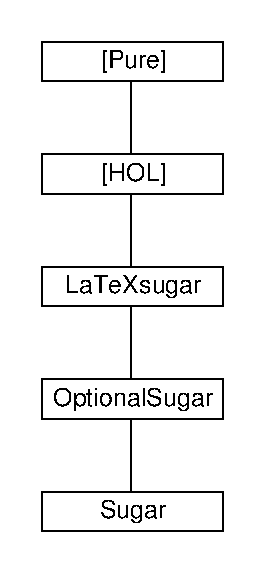
\includegraphics[width=\textwidth,height=0.95\textheight,keepaspectratio]{session_graph}
\end{center}
\caption{Theory Dependency Graph\label{theory-deps}}
\end{figure}

\newpage
%
\begin{isabellebody}%
\def\isabellecontext{a{\isadigit{6}}}%
\isamarkupfalse%
%
\isamarkupsubsection{Optimising Compiler Verification%
}
\isamarkuptrue%
%
\begin{isamarkuptext}%
Section 3.3 of the Isabelle tutorial describes an expression compiler for a stack machine. In this exercise we will build and verify an optimising expression compiler for a register machine.%
\end{isamarkuptext}%
\isamarkuptrue%
%
\begin{isamarkuptext}%
\subsubsection*{The Source Language: Expressions}%
\end{isamarkuptext}%
\isamarkuptrue%
%
\begin{isamarkuptext}%
The arithmetic expressions we will work with consist of variables, constants, and an arbitrary binary operator \isa{oper}.%
\end{isamarkuptext}%
\isamarkuptrue%
\isacommand{consts}\ oper\ {\isacharcolon}{\isacharcolon}\ {\isachardoublequote}nat\ {\isasymRightarrow}\ nat\ {\isasymRightarrow}\ nat{\isachardoublequote}\isanewline
\isanewline
\isamarkupfalse%
\isacommand{types}\ var\ {\isacharequal}\ string\isanewline
\isanewline
\isamarkupfalse%
\isacommand{datatype}\ exp\ {\isacharequal}\ \isanewline
\ \ \ \ Const\ nat\ \isanewline
\ \ {\isacharbar}\ Var\ var\isanewline
\ \ {\isacharbar}\ Op\ exp\ exp\isamarkupfalse%
%
\begin{isamarkuptext}%
The state in which an expression is evaluated is modelled by an {\em environment} function that maps variables to constants.%
\end{isamarkuptext}%
\isamarkuptrue%
\isacommand{types}\ env\ {\isacharequal}\ {\isachardoublequote}var\ {\isasymRightarrow}\ nat{\isachardoublequote}\isamarkupfalse%
%
\begin{isamarkuptext}%
Define a function \isa{value} that evaluates an expression in a given environment.%
\end{isamarkuptext}%
\isamarkuptrue%
\isacommand{consts}\ value\ {\isacharcolon}{\isacharcolon}\ {\isachardoublequote}exp\ {\isasymRightarrow}\ env\ {\isasymRightarrow}\ nat{\isachardoublequote}\isamarkupfalse%
%
\begin{isamarkuptext}%
\subsubsection*{The Register Machine}%
\end{isamarkuptext}%
\isamarkuptrue%
%
\begin{isamarkuptext}%
As the name suggests, a register machine uses a collection of registers to store intermediate results. There exists a special register, called the accumulator, that serves as an implicit argument to each instruction. The rest of the registers make up the register file, and can be randomly accessed using an index.%
\end{isamarkuptext}%
\isamarkuptrue%
\isacommand{types}\ regIndex\ {\isacharequal}\ nat\isanewline
\isanewline
\isamarkupfalse%
\isacommand{datatype}\ cell\ {\isacharequal}\ \isanewline
\ \ \ \ Acc\isanewline
\ \ {\isacharbar}\ Reg\ regIndex\isamarkupfalse%
%
\begin{isamarkuptext}%
The state of the register machine is denoted by a function that maps storage cells to constants.%
\end{isamarkuptext}%
\isamarkuptrue%
\isacommand{types}\ state\ {\isacharequal}\ {\isachardoublequote}cell\ {\isasymRightarrow}\ nat{\isachardoublequote}\isamarkupfalse%
%
\begin{isamarkuptext}%
The instruction set for the register machine is defined as follows:%
\end{isamarkuptext}%
\isamarkuptrue%
\isacommand{datatype}\ instr\ {\isacharequal}\ \isanewline
\ \ LI\ nat\ \ \ \ \ \ \ \ \isanewline
\ \ %
\isamarkupcmt{Load Immediate: loads a constant into the accumulator.%
}
\ \isanewline
{\isacharbar}\ LOAD\ regIndex\ \isanewline
\ \ %
\isamarkupcmt{Loads the contents of a register into the accumulator.%
}
\isanewline
{\isacharbar}\ STORE\ regIndex\ \isanewline
\ \ %
\isamarkupcmt{Saves the contents of the accumulator in a register.%
}
\ \isanewline
{\isacharbar}\ OPER\ regIndex\ \isanewline
\ \ %
\isamarkupcmt{Performs the binary operation \isa{oper}.%
}
\isanewline
\ \ \ \ %
\isamarkupcmt{The first argument is taken from a register.%
}
\isanewline
\ \ \ \ %
\isamarkupcmt{The second argument is taken from the accumulator.%
}
\ \isanewline
\ \ \ \ %
\isamarkupcmt{The result of the computation is stored in the accumulator.%
}
\isamarkupfalse%
%
\begin{isamarkuptext}%
A program is a list of such instructions. The result of running a program is a change of state of the register machine. Define a function \isa{exec} that models this.%
\end{isamarkuptext}%
\isamarkuptrue%
\isacommand{consts}\ exec\ {\isacharcolon}{\isacharcolon}\ {\isachardoublequote}state\ {\isasymRightarrow}\ instr\ list\ {\isasymRightarrow}\ state{\isachardoublequote}\isamarkupfalse%
%
\begin{isamarkuptext}%
\subsubsection*{Compilation}%
\end{isamarkuptext}%
\isamarkuptrue%
%
\begin{isamarkuptext}%
The task now is to translate an expression into a sequence of instructions that computes it. At the end of execution, the result should be stored in the accumulator.

Before execution, the values of each variable need to be stored somewhere in the register file. A {\it mapping} function maps variables to positions in the register file.%
\end{isamarkuptext}%
\isamarkuptrue%
\isacommand{types}\ map\ {\isacharequal}\ {\isachardoublequote}var\ {\isasymRightarrow}\ regIndex{\isachardoublequote}\isamarkupfalse%
%
\begin{isamarkuptext}%
Define a function \isa{cmp} that compiles an expression into a sequence of instructions. The evaluation should proceed in a bottom-up depth-first manner.

State and prove a theorem expressing the correctness of \isa{cmp}.

Hints:
\begin{itemize}
  \item The compilation function is dependent on the mapping function.
  \item The compilation function needs some way of storing intermediate results. It should be clever enough to reuse registers it no longer needs.
  \item It may be helpful to assume that at each recursive call, compilation is only allowed to use registers with indices greater than a given value to store intermediate results.
\end{itemize}%
\end{isamarkuptext}%
\isamarkuptrue%
%
\begin{isamarkuptext}%
\subsubsection*{Compiler Optimisation: Common Subexpressions}%
\end{isamarkuptext}%
\isamarkuptrue%
%
\begin{isamarkuptext}%
In the previous section, the compiler \isa{cmp} was allowed to evaluate a subexpression every time it occurred. In situations where arithmetic operations are costly, one may want to compute commonly occurring subexpressions only once.

For example, to compute \isa{{\isacharparenleft}a\ op\ b{\isacharparenright}\ op\ {\isacharparenleft}a\ op\ b{\isacharparenright}}, \isa{cmp} was allowed three calls to \isa{oper}, when only two were needed.

Develop an optimised compiler \isa{optCmp}, that evaluates every commonly occurring subexpression only once. Prove its correctness.%
\end{isamarkuptext}%
\isamarkuptrue%
\isamarkupfalse%
\end{isabellebody}%
%%% Local Variables:
%%% mode: latex
%%% TeX-master: "root"
%%% End:


%%% Local Variables:
%%% mode: latex
%%% TeX-master: "root"
%%% End:


\newpage
\nocite{*}
\bibliographystyle{abbrv}
\bibliography{root}

\end{document}
